\documentclass[12pt,a4paper]{report}

% --- Paquets bàsics ---
\usepackage[catalan]{babel}
\usepackage[utf8]{inputenc}
\usepackage[T1]{fontenc}
\usepackage{lmodern}
\usepackage{geometry}
\usepackage{setspace}
\usepackage{graphicx}
\usepackage[hidelinks]{hyperref}
\usepackage{amsmath}
\usepackage{amsfonts}
\usepackage{amssymb}
\usepackage{float}
\usepackage{listings}
\usepackage{xcolor}
\usepackage{caption}
\usepackage{wrapfig}


\lstdefinelanguage{CSharp}{
  language=[Sharp]C
}

\lstset{
  basicstyle=\ttfamily\footnotesize,
  breaklines=true,
  breakatwhitespace=false,
  postbreak=\mbox{\textcolor{red}{$\hookrightarrow$}\space},
  captionpos=b,
  frame=single,
  framerule=0.5pt,
  rulecolor=\color{gray!60},
  aboveskip=6pt,
  belowskip=6pt,
  keywordstyle=\color{blue},
  commentstyle=\color{gray},
  stringstyle=\color{teal},
  showstringspaces=false,
  tabsize=2
}
\begin{document}

\chapter{Disseny del sistema d'automatització}
En aquest capítol es descriu el disseny del sistema d'automatització per al control de la planta. Es detallen els components principals, la seva interacció i les tecnologies utilitzades.

\section{GRAFCET}

El control de la planta s'ha dissenyat mitjançant la metodologia GRAFCET, que permet definir el comportament seqüencial del sistema a partir d'etapes i transicions.

A nivell de disseny, el sistema s'ha dividit en diferents GRAFCETs amb l'objectiu de separar la lògica de procés del control d'actuadors i facilitar tant la implementació com el manteniment.

\begin{itemize}
\item GRAFCET general
\item GRAFCETs de classificació (A, B i C)
\item GRAFCET d'evacuació
\item GRAFCETs d'actuadors
\item GRAFCETs de control (marxa/aturada, selector, emergència i avaria)
\end{itemize}

A més, es defineixen una sèrie de condicions globals que es poden observar en la taula \ref{tab:condicions_control}:


\begin{table}[H]
\centering
\renewcommand{\arraystretch}{1.5}

\begin{tabular}{|p{3.5cm}|p{9.8cm}|}
\hline
\textbf{Condició} & \textbf{Descripció} \\
\hline

\texttt{CI} &
Verifica les condicions inicials del sistema. Tots els sensors de presència han d'estar desactivats i els transelevadors han de trobar-se en la seva posició inicial correcta (S4, S8, SH1 i SV1 actius) \footnote{Els sensors de presència de les estanteries no es tenen en compte en aquesta verificació, ja que el sistema permet iniciar-se amb peces ja emmagatzemades}.  \\


\hline

\texttt{COND\_AUTO} &
Indica que el sistema es troba en mode automàtic, amb el selector en posició automàtica, el sistema sense emergència activa i el botó de pausa desactivat. \\

\hline

\texttt{COND\_MANUAL} &
Determina que el sistema es troba funcionant en mode manual. \\
\hline

\texttt{CI\_Actuators} &
Comprova que tots els actuadors i GRAFCETs associats es troben en el seu estat inicial segur abans de permetre certes transicions del sistema. \\

\hline

\end{tabular}

\caption{Condicions globals de control del sistema}
\label{tab:condicions_control}

\end{table}

\subsection{GRAFCET general}
\begin{wrapfigure}[20]{r}{0.42\textwidth}
\vspace{-10pt}

\centering
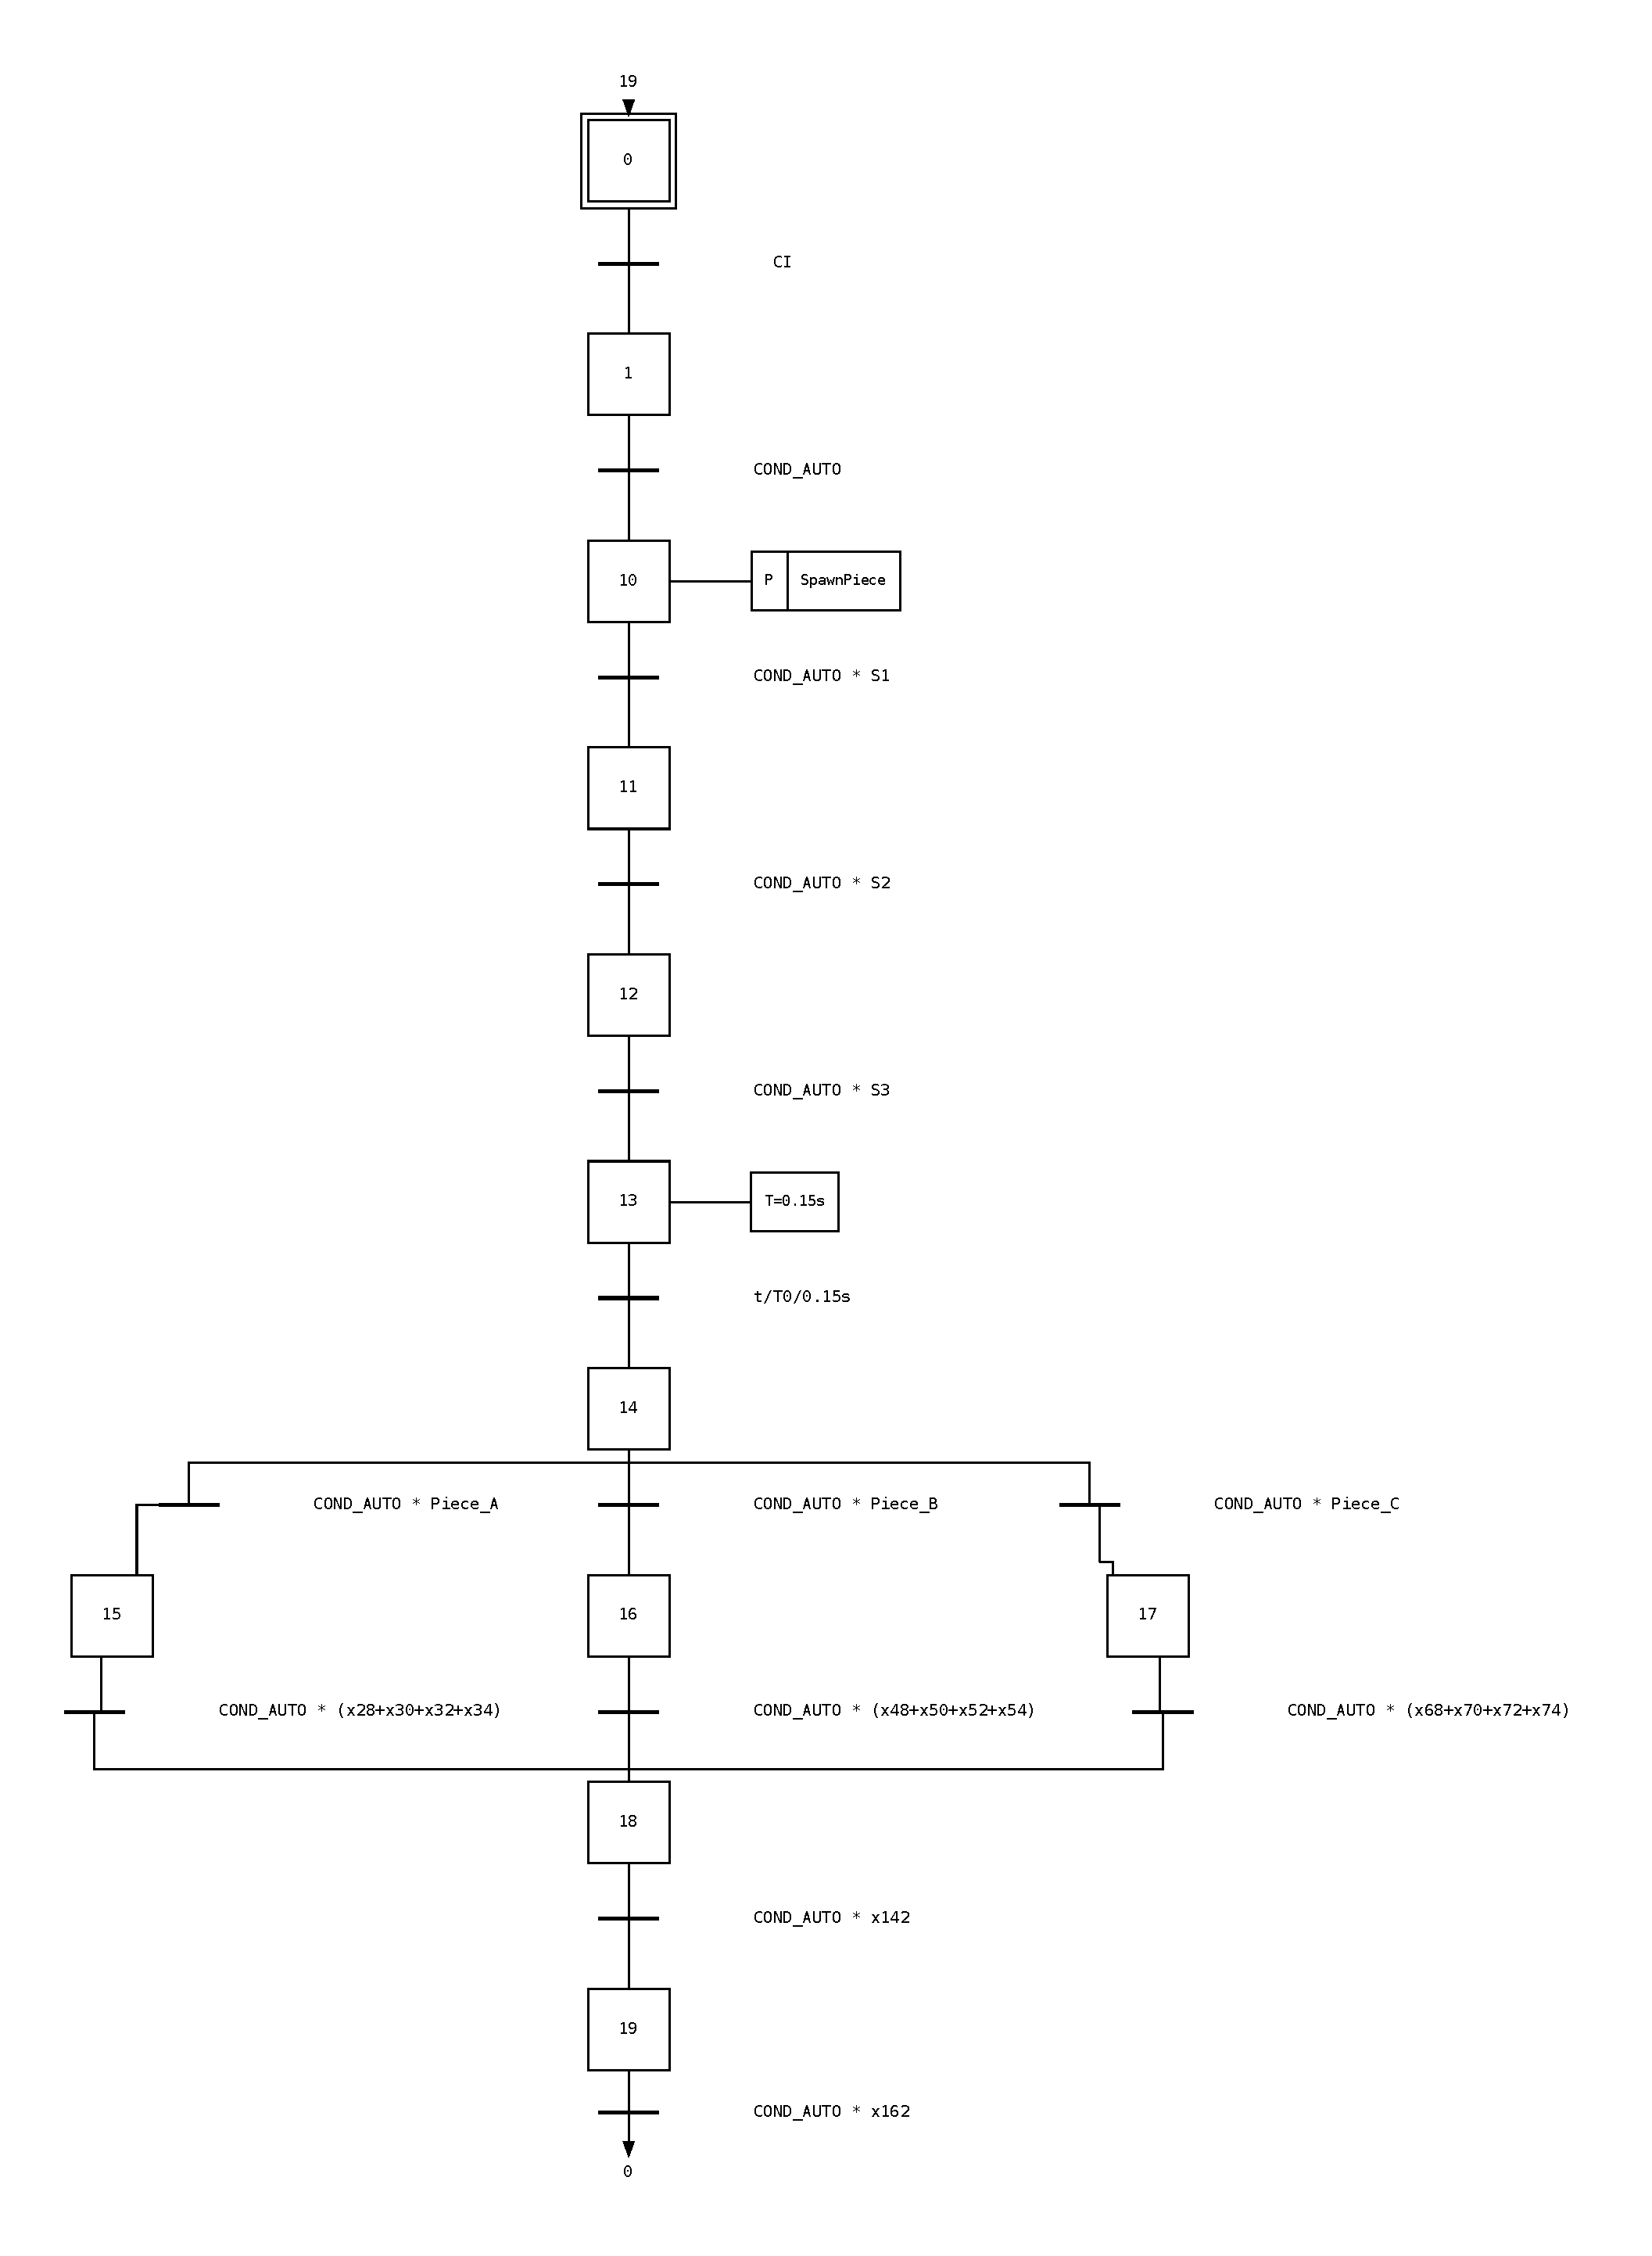
\includegraphics[width=\linewidth]{PDF_GRAFCET/G0.pdf}
\caption{GRAFCET general del sistema (G0)}
\label{fig:grafcet_general}

\vspace{-15pt}
\end{wrapfigure}
El GRAFCET general (G0, Figura \ref{fig:grafcet_general}) defineix el flux principal del procés automàtic. En aquest cas, no es controlen directament actuadors, sinó que es coordinen els diferents subprocessos del sistema.




\begin{itemize}
\item \textbf{E0:} Estat inicial. Comprovació de condicions inicials (CI).
\item \textbf{E10-E12:} Entrada de peça mitjançant sensors:
  \begin{itemize}
  \item S1: presència a la cinta
  \item S2: detecció del tipus de peça
  \item S3: presència a la plataforma del transelevador
  \end{itemize}
    L'estat 10 permet fer apareixer les peces a la cinta de forma controlada.
\item \textbf{E13:} Introdueix una temporització de 0.15 segons necessària per assegurar que la peça estigui correctament situada sobre la plataforma

\item \textbf{E14:} Decisió segons tipus de peça:
  \begin{itemize}
  \item Peça A → E15
  \item Peça B → E16
  \item Peça C → E17
  \end{itemize}

\item \textbf{E15-E17:} Espera la finalització de la col·locació de la peça (condicions sobre x28, x48, x68...).

\item \textbf{E18-E19:} Retorn del transelevador a posició inicial (condicions x142 i x162).

\end{itemize}



\subsection{GRAFCET de classificació}

S'han fet 3 programes per dipositar les peces a la posició corresponent del magatzem. Aques programes es correponen amb els GRAFCET G20 (Figura \ref{fig:grafcet_clasificacion}), G40 i G60 i col·loquen les peces a les estanteries A, B i C respectivament.


Prenent com a exemple l'estanteria A:

\begin{itemize}
\item \textbf{E20:} Entrada al GRAFCET de classificació.
\item \textbf{E21:} Temporització de posicionament vertical (T2\_A).
\item \textbf{E22:} Decisió segons el comptador de peces de l'estanteria A (C\_A mod 3) passar a una de les tres possibles estanteries (E23, E24 o E25).:
  \begin{itemize}
  \item 0 → E23
  \item 1 → E24
  \item 2 → E25
  \end{itemize}

\item \textbf{E26:} Temporització T1 per assegurar el dipòsit.
\item \textbf{E27:} Increment del comptador (C\_A = C\_A + 1) com acció impulsional  (només s'executa una vegada al entrar en aquesta etapa.)

\item \textbf{Possible moviment dintre de l'estantería:}
\begin{itemize}
\item C\_A mod 3 $\neq$ 0 → E28 (retorn)
\item C\_A = 3 → E29-E30 (avanç d'una fila)
\item C\_A = 6 → E31-E32 (avanç de dues files)
\item C\_A = 9 → E33-E34 (activació evacuació, es realitza un reset del comptador de l'estantería i es suma un al comptador general d'evacuacions de cada peça)
\end{itemize}
\end{itemize}


\begin{figure}
  \centering
    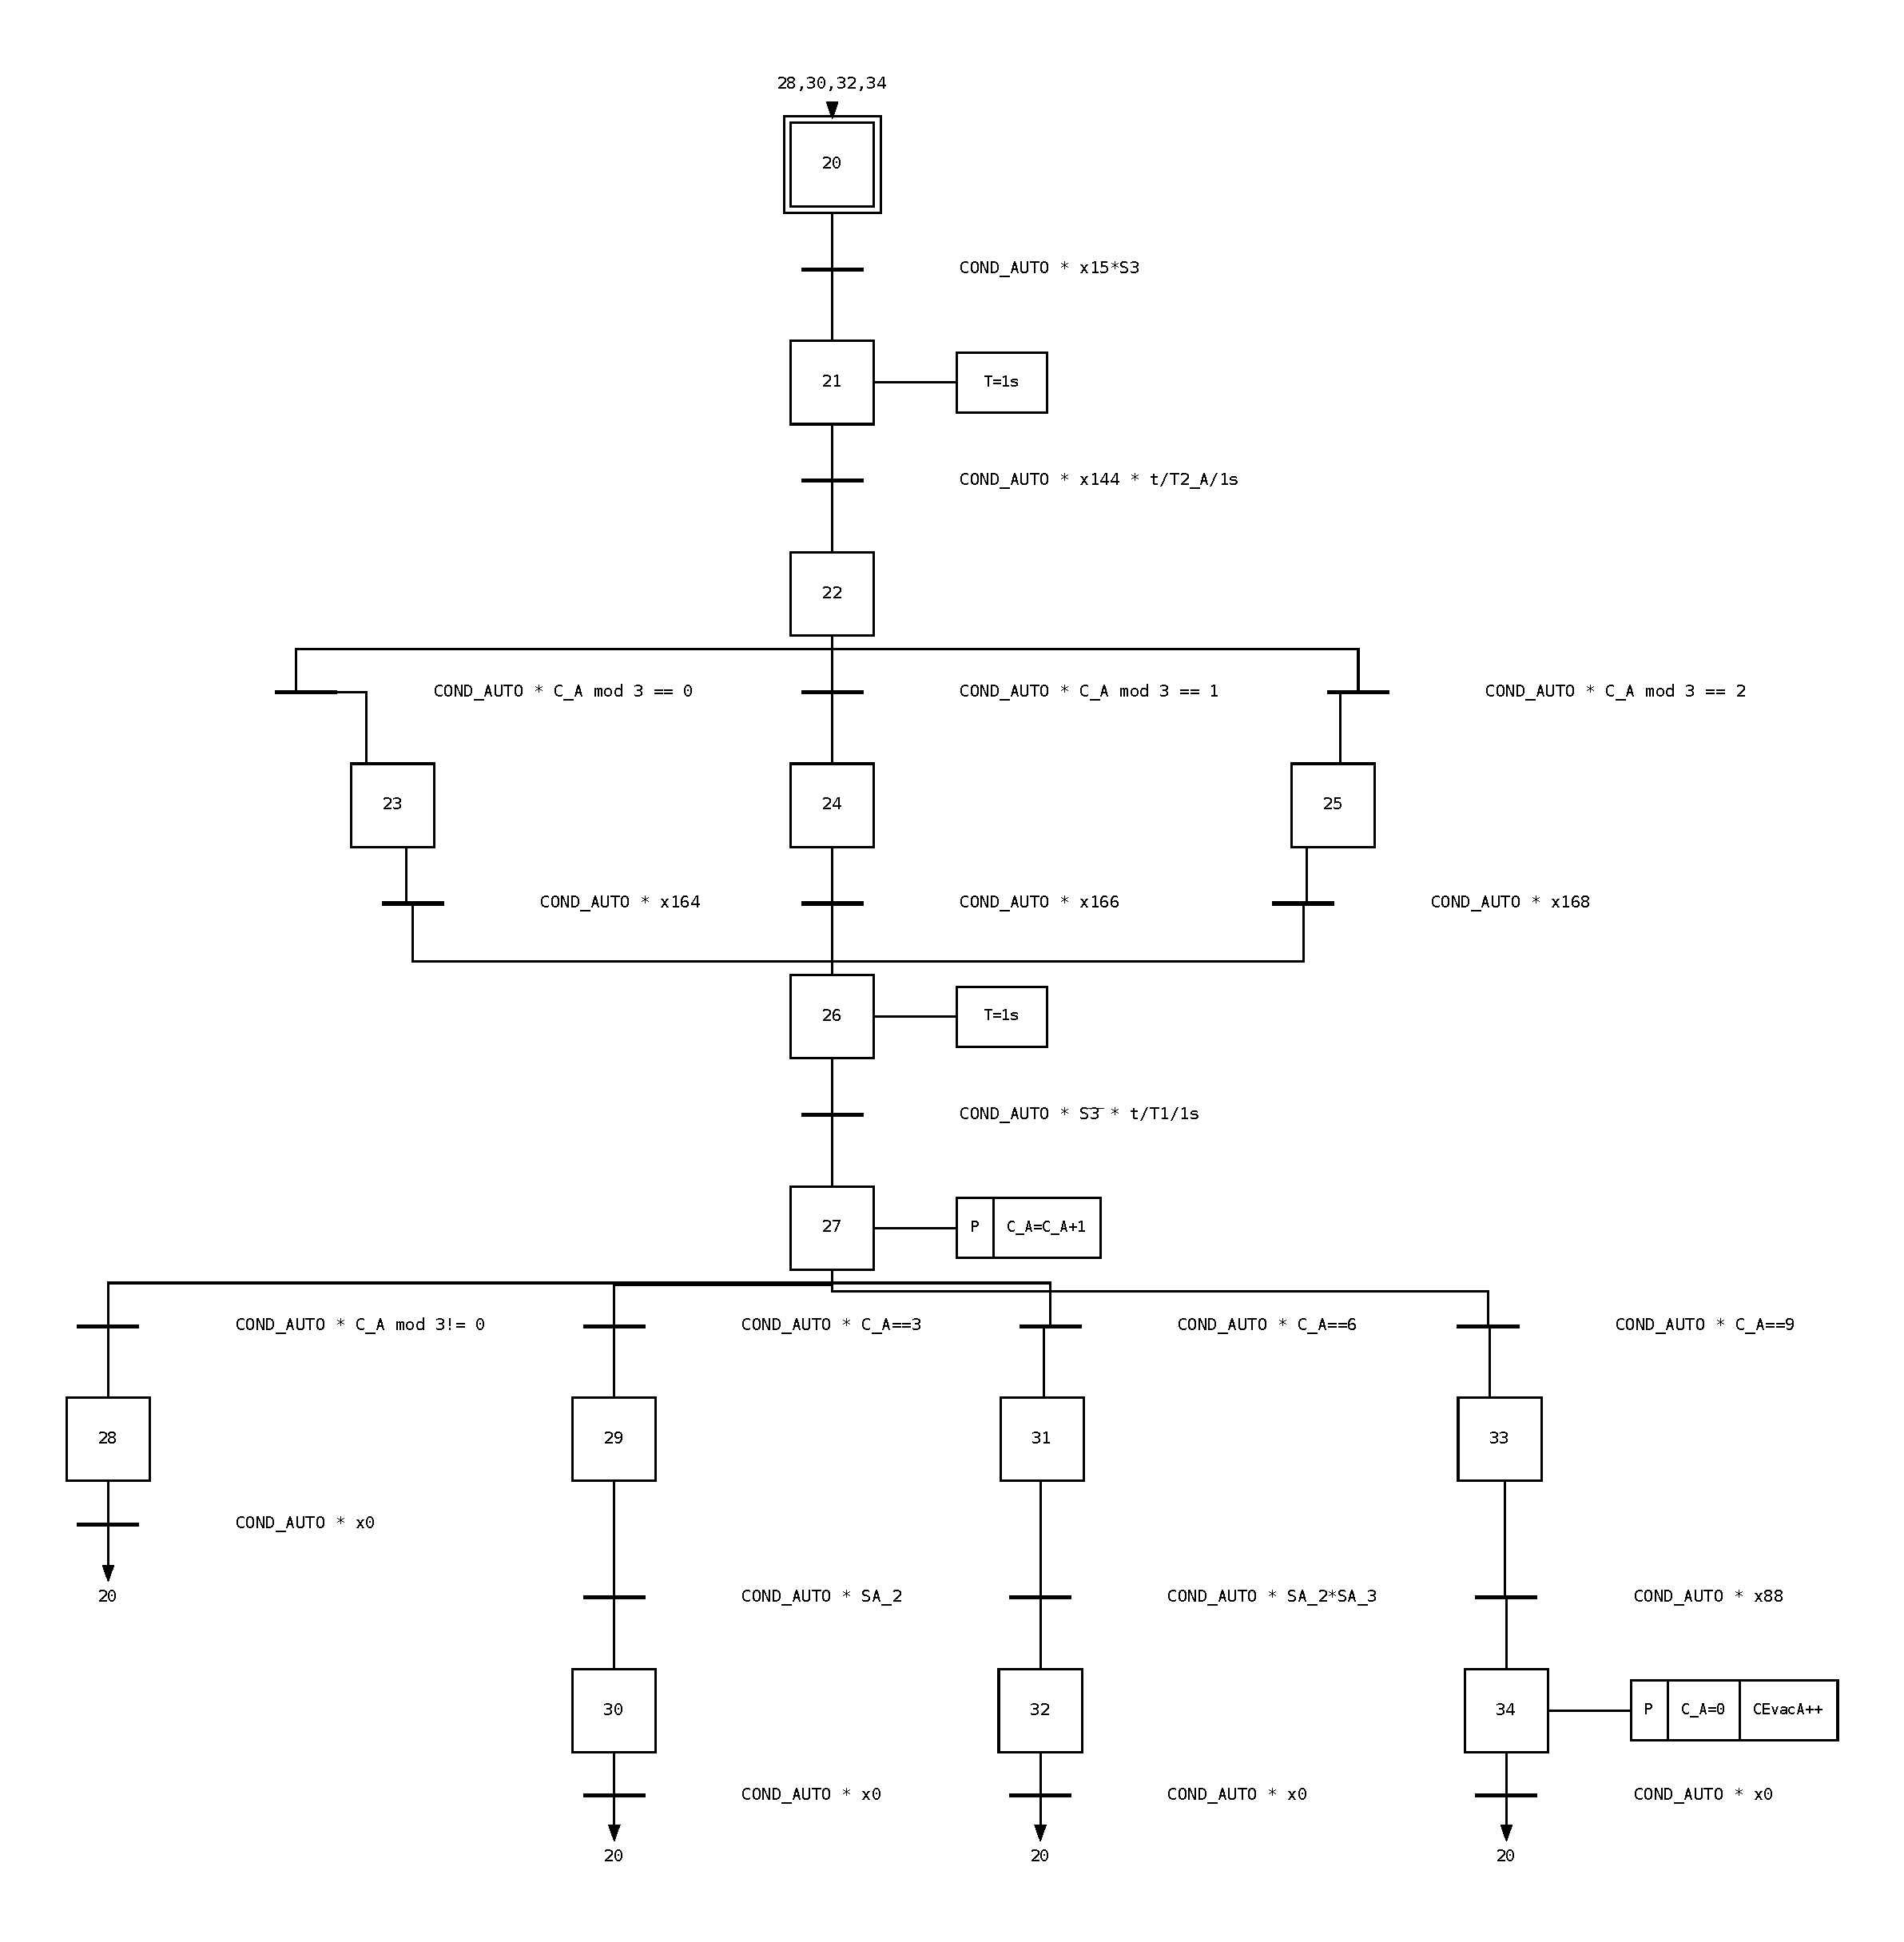
\includegraphics[width=0.5\textwidth]{PDF_GRAFCET/G20.pdf}
  \caption{GRAFCET de classificació d'estanteria A}
  \label{fig:grafcet_clasificacion}
\end{figure}



\subsection{GRAFCET d'evacuació}

\begin{figure}[H]

\begin{minipage}[t]{0.60\textwidth}
\vspace{0pt}
El GRAFCET d'evacuació (G80, Figura \ref{fig:grafcet_evacuacion}) gestiona el buidatge de les estanteries.


El procés és el següent:

\begin{itemize}
\item \textbf{E80:} Determinació de l'estanteria origen que ha estat plena. Com el sistema esta preparat per rebre una peça per cicle, és impossible que s'activin l'estat E33, E53 o E73 a la vegada.
\item \textbf{E81-E83:} Quan una etapa de les anteriors mencionades s'activi, aquest programa comprovorà quina posició vertical ha de prendre el transelevador 2
\item \textbf{E84:} Selecció segons tipus de peça
\item \textbf{E85-E87:} Transferència de peces amb els rodets de plataforma i rodets d'estanteria
\item \textbf{E88-E90:} Moviment cap a cinta d'evacuació
\item \textbf{E91-E92:} Descàrrega i retorn a estat inicial
\end{itemize}

\end{minipage}
\hspace{0.03\textwidth}\begin{minipage}[t]{0.36\textwidth}

\vspace{0pt}

\centering
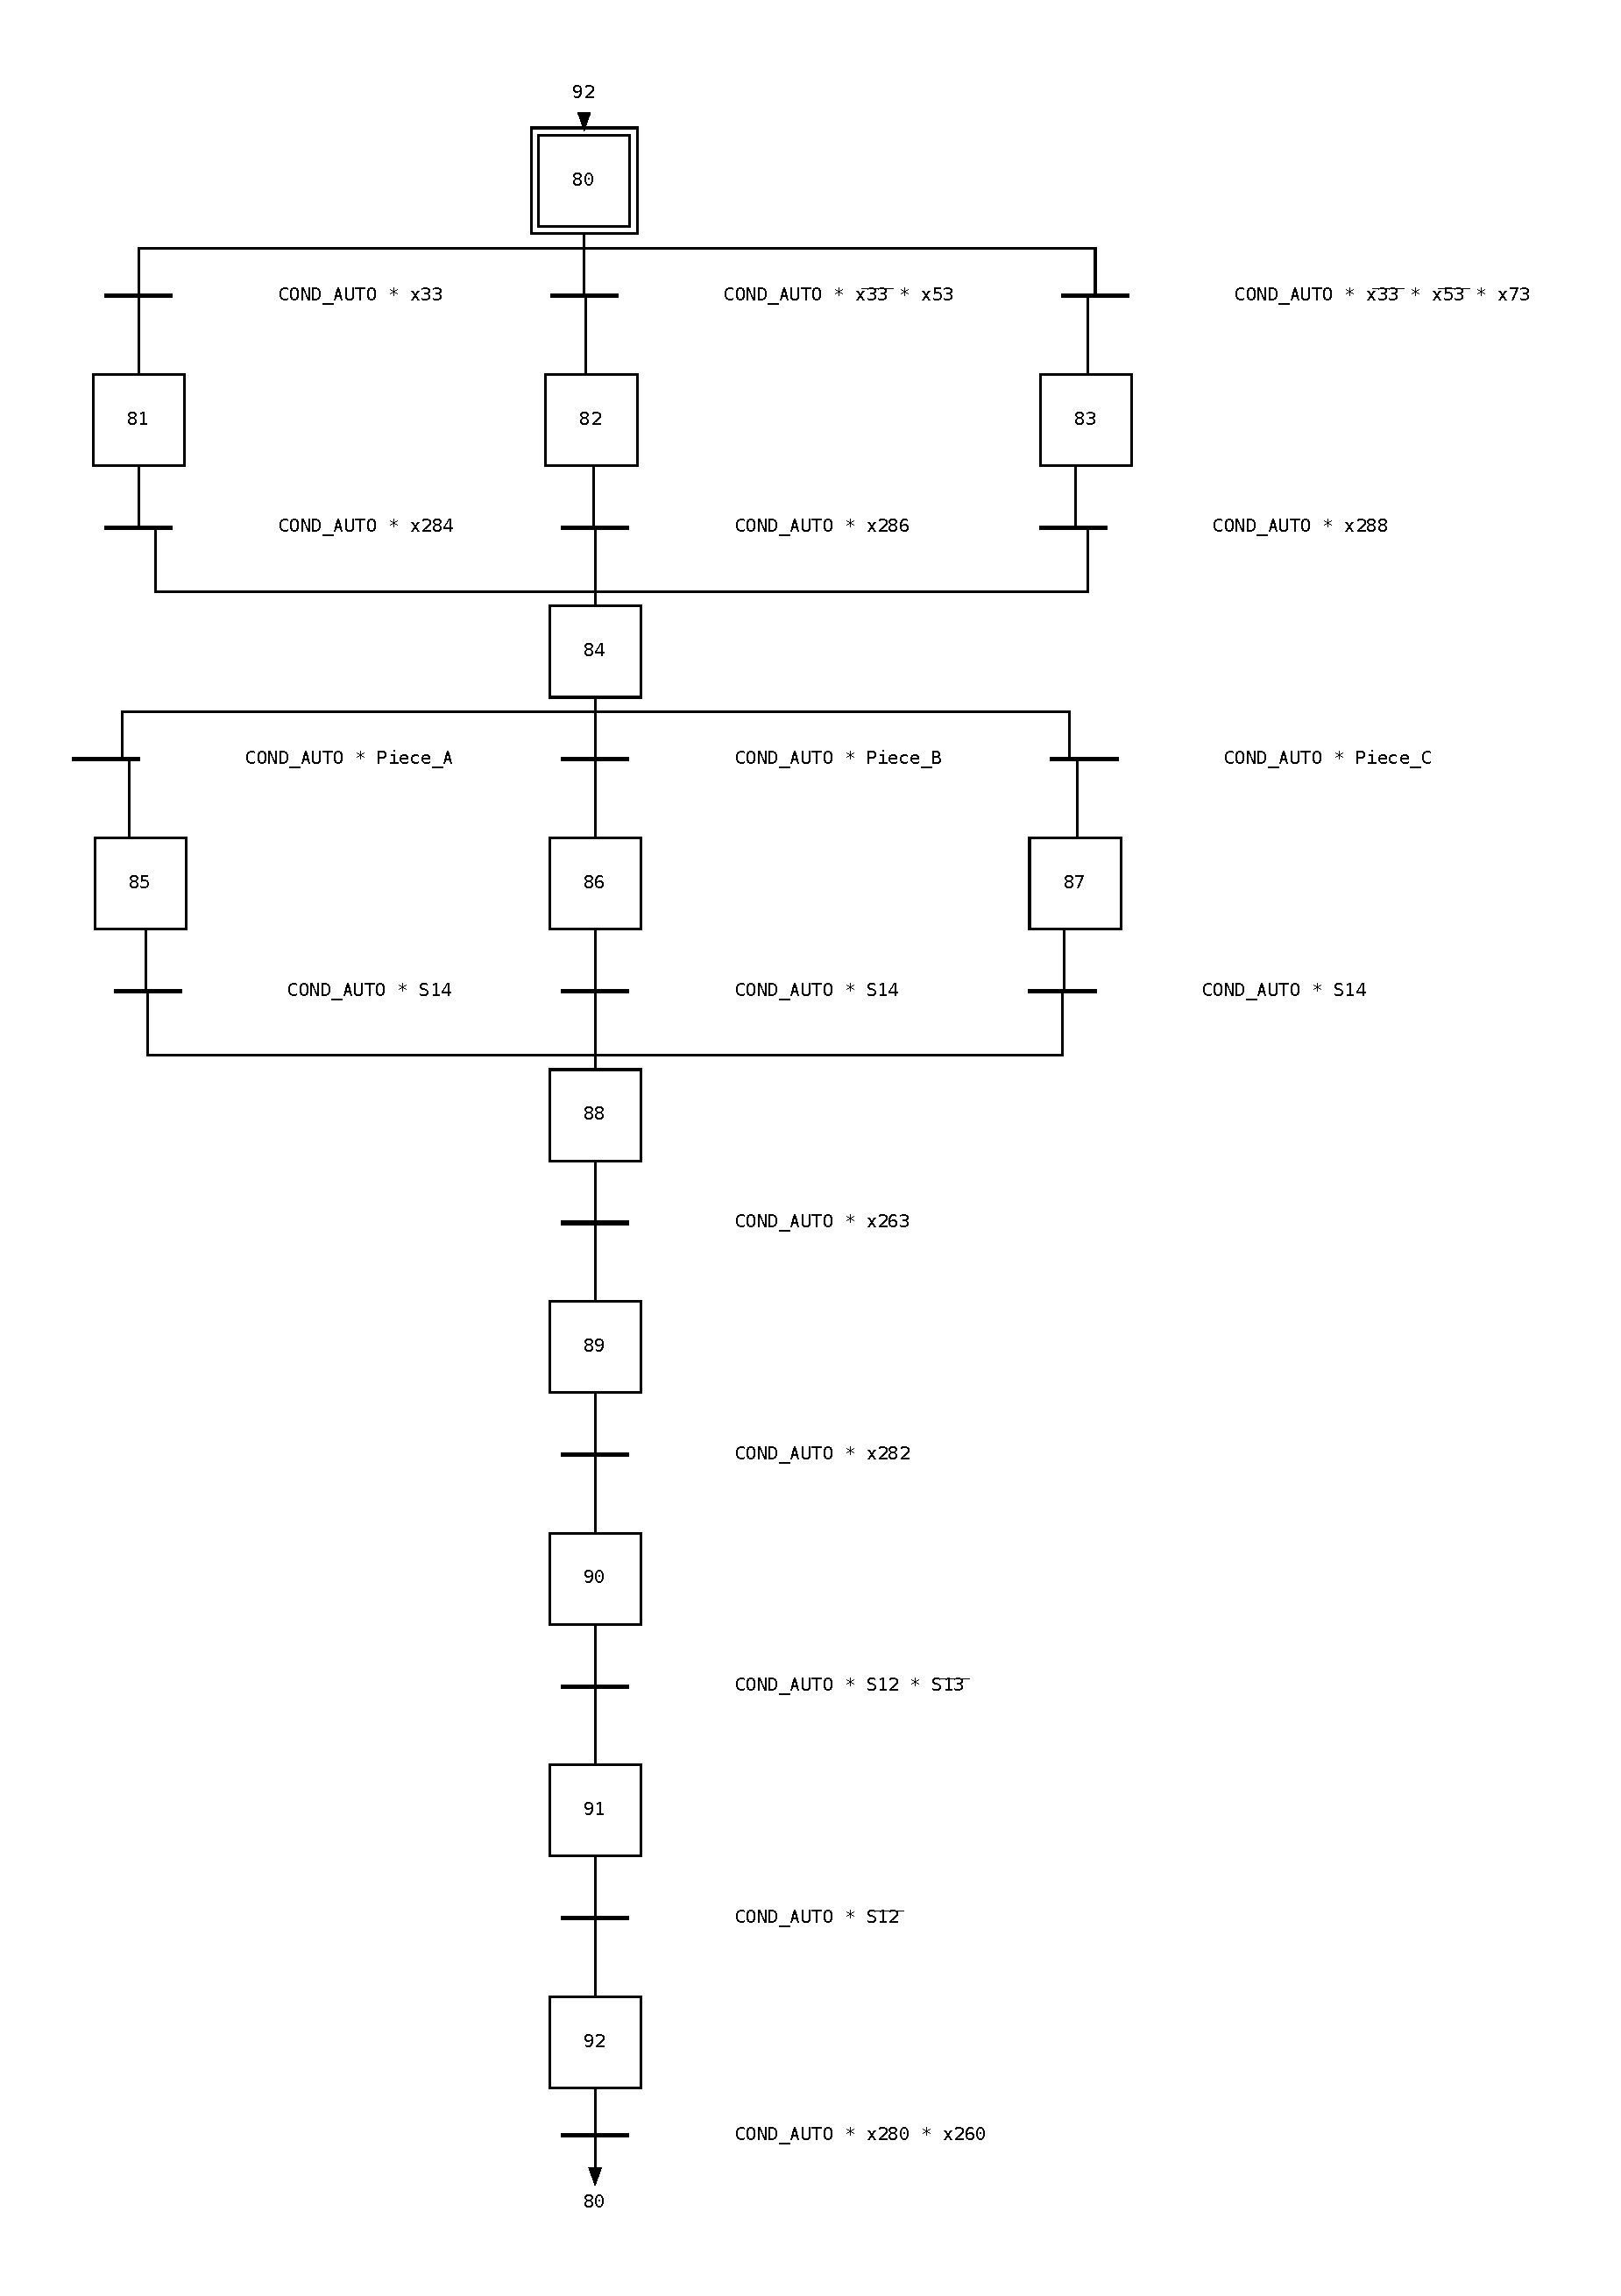
\includegraphics[width=\textwidth]{PDF_GRAFCET/G80.pdf}

\caption{GRAFCET d'evacuació del sistema (G80)}
\label{fig:grafcet_evacuacion}

\end{minipage}

\end{figure}


\subsection{GRAFCET Actuadors}

\begin{wrapfigure}[10]{r}{0.3\textwidth} 

\vspace{-10pt}

\centering
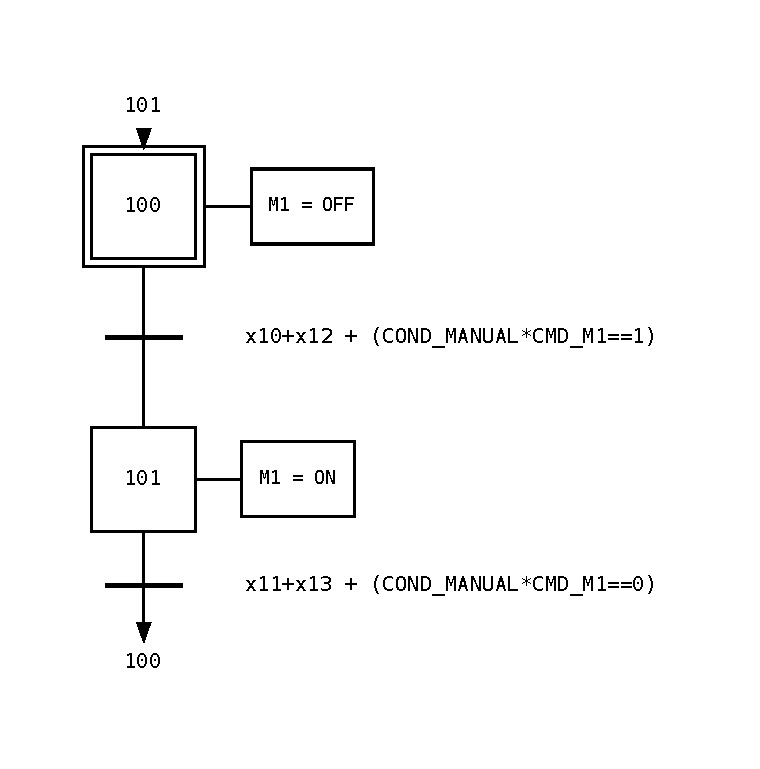
\includegraphics[width=0.5\textwidth]{PDF_GRAFCET/G100.pdf}
\caption{GRAFCET de control de cinta transportadora}
\label{fig:grafcet_cinta}
\vspace{-10pt}

\end{wrapfigure}

Els actuadors es controlen mitjançant GRAFCETs independents, que interpreten els estats actius del sistema:
\begin{itemize}
\item \textbf{Cintes (G100, G3G0) $\rightarrow$ Amb dos estats de funcionament (Figura \ref{fig:grafcet_cinta}):}
  \begin{itemize}
  \item Estat STOP
  \item Estat RUN
  \end{itemize}
\item \textbf{Rodets d'estanteria (G180):}
Funcionament equivalent a les cintes però amb direcció específica.
\item \textbf{Rodets de plataforma (G120, G240) $\rightarrow$ Amb tres estats de funcionament (Figura \ref{fig:grafcet_rodets}):}
\begin{itemize}
\item STOP
\item Moviment sentit positiu
\item Moviment sentit negatiu
\end{itemize}
Com a decisió de disseny, és obligatori passar per STOP per canviar de direcció, fet que succeeix en el procès automàtic i s'ha implementat en el mode manual.

\begin{figure}[H]
\centering
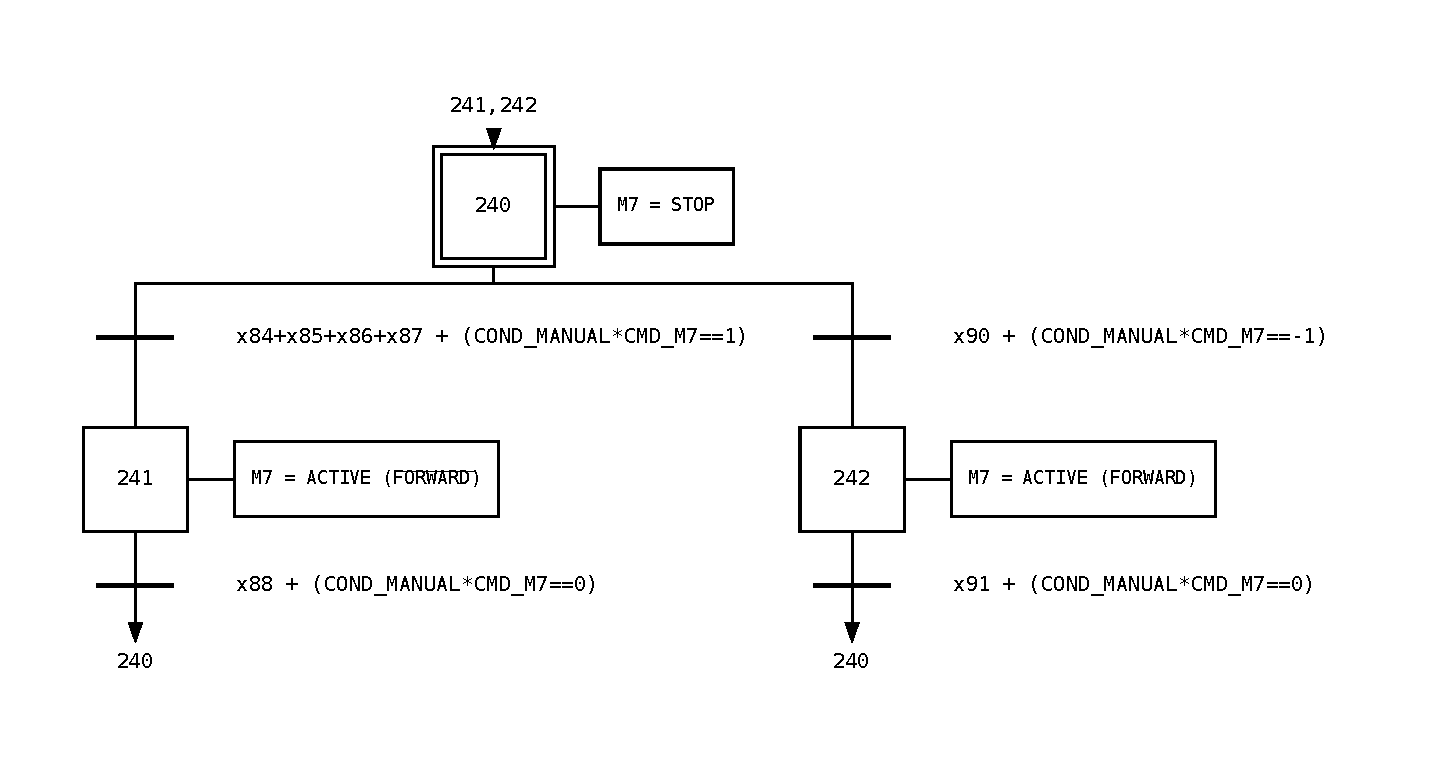
\includegraphics[width=0.7\textwidth]{PDF_GRAFCET/G240.pdf}
\caption{GRAFCET de control de rodets amb canvi de direcció}
\label{fig:grafcet_rodets}
\end{figure}

\item \textbf{Transelevadors (Figura \ref{fig:grafcet_transelevador}):}
\begin{itemize}

\item \textbf{Transelevador 1 (G140, G160):} disposa de 4 posicions verticals i 4 horitzontals, cadascuna amb el seu estat de confirmació mitjançant sensors. Els GRAFCETs associats consten de 9 estats:
\begin{itemize}
\item 1 estat inicial (repòs)
\item 4 estats de moviment (un per cada posició)
\item 4 estats de confirmació de posició
\end{itemize}

\item \textbf{Transelevador 2 (E260, E280):} presenta una configuració reduïda. El moviment vertical funciona de manera anàloga al Transelevador 1, mentre que el moviment horitzontal només disposa de 2 posicions. En aquest cas, el GRAFCET horitzontal es simplifica i l'estat inicial també actua com a estat de confirmació per a la posició base.
\end{itemize}


Un cop el transelevador arriba a una posició, el sistema entra en un \textbf{estat de confirmació}, que valida que el moviment s'ha completat correctament mitjançant els sensors corresponents.

Per garantir un comportament robust i evitar reactivacions no desitjades, la sortida d'aquest estat segueix dues regles fonamentals:

\begin{itemize}
\item El sistema només abandona l'estat de confirmació quan es rep una \textbf{nova comanda diferent} de la que ha provocat el moviment.
\item En el cas de la \textbf{posició inicial}, es força que la comanda deixi de ser vàlida un cop assolida la posició, assegurant que el sistema es manté en repòs fins a una nova acció de l'usuari.
\end{itemize}
\end{itemize}


\begin{figure}[H]
\centering

\begin{minipage}{0.6\textwidth}
\centering
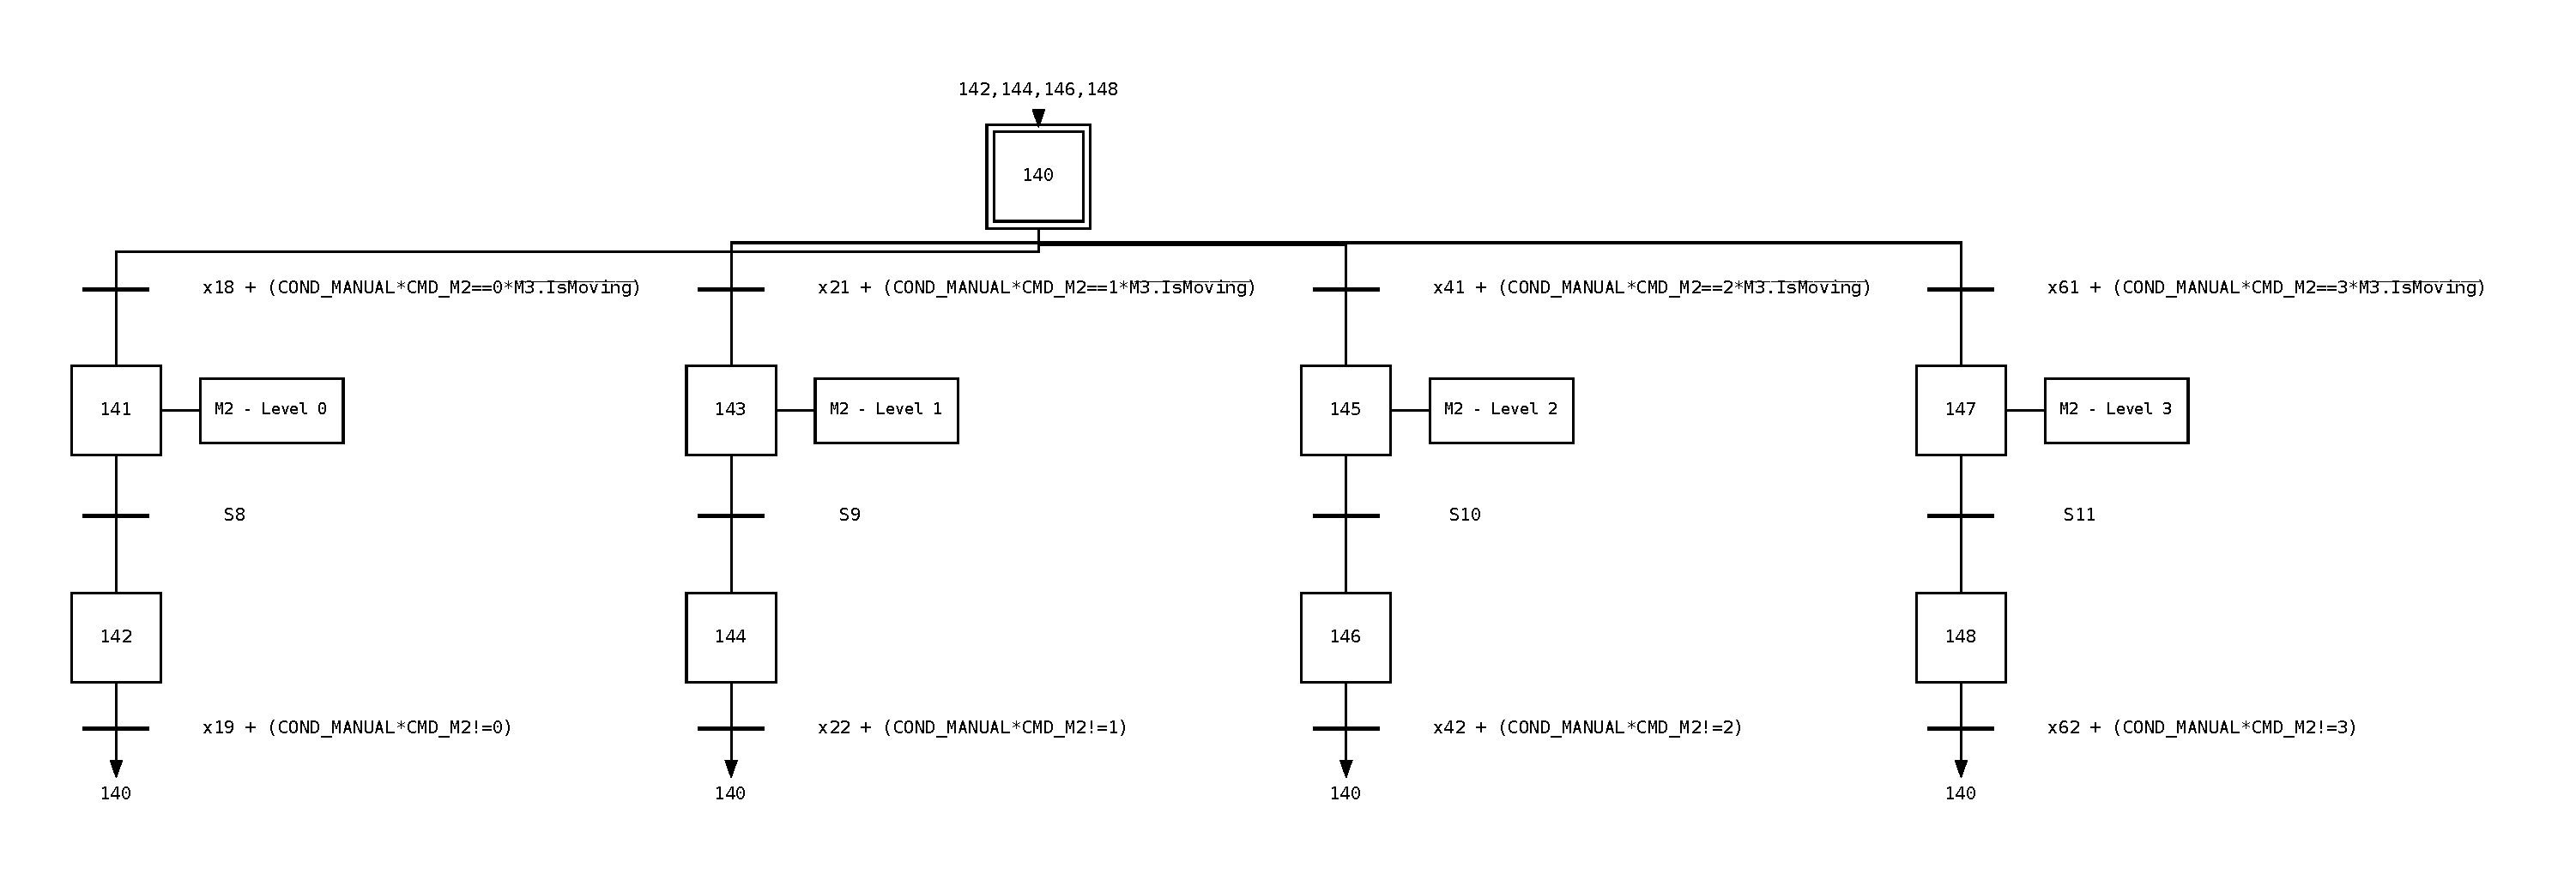
\includegraphics[width=\textwidth]{PDF_GRAFCET/G140.pdf}
\vspace{4pt}
\small (a) Moviment vertical
\end{minipage}
\hfill
\begin{minipage}{0.6\textwidth}
\centering
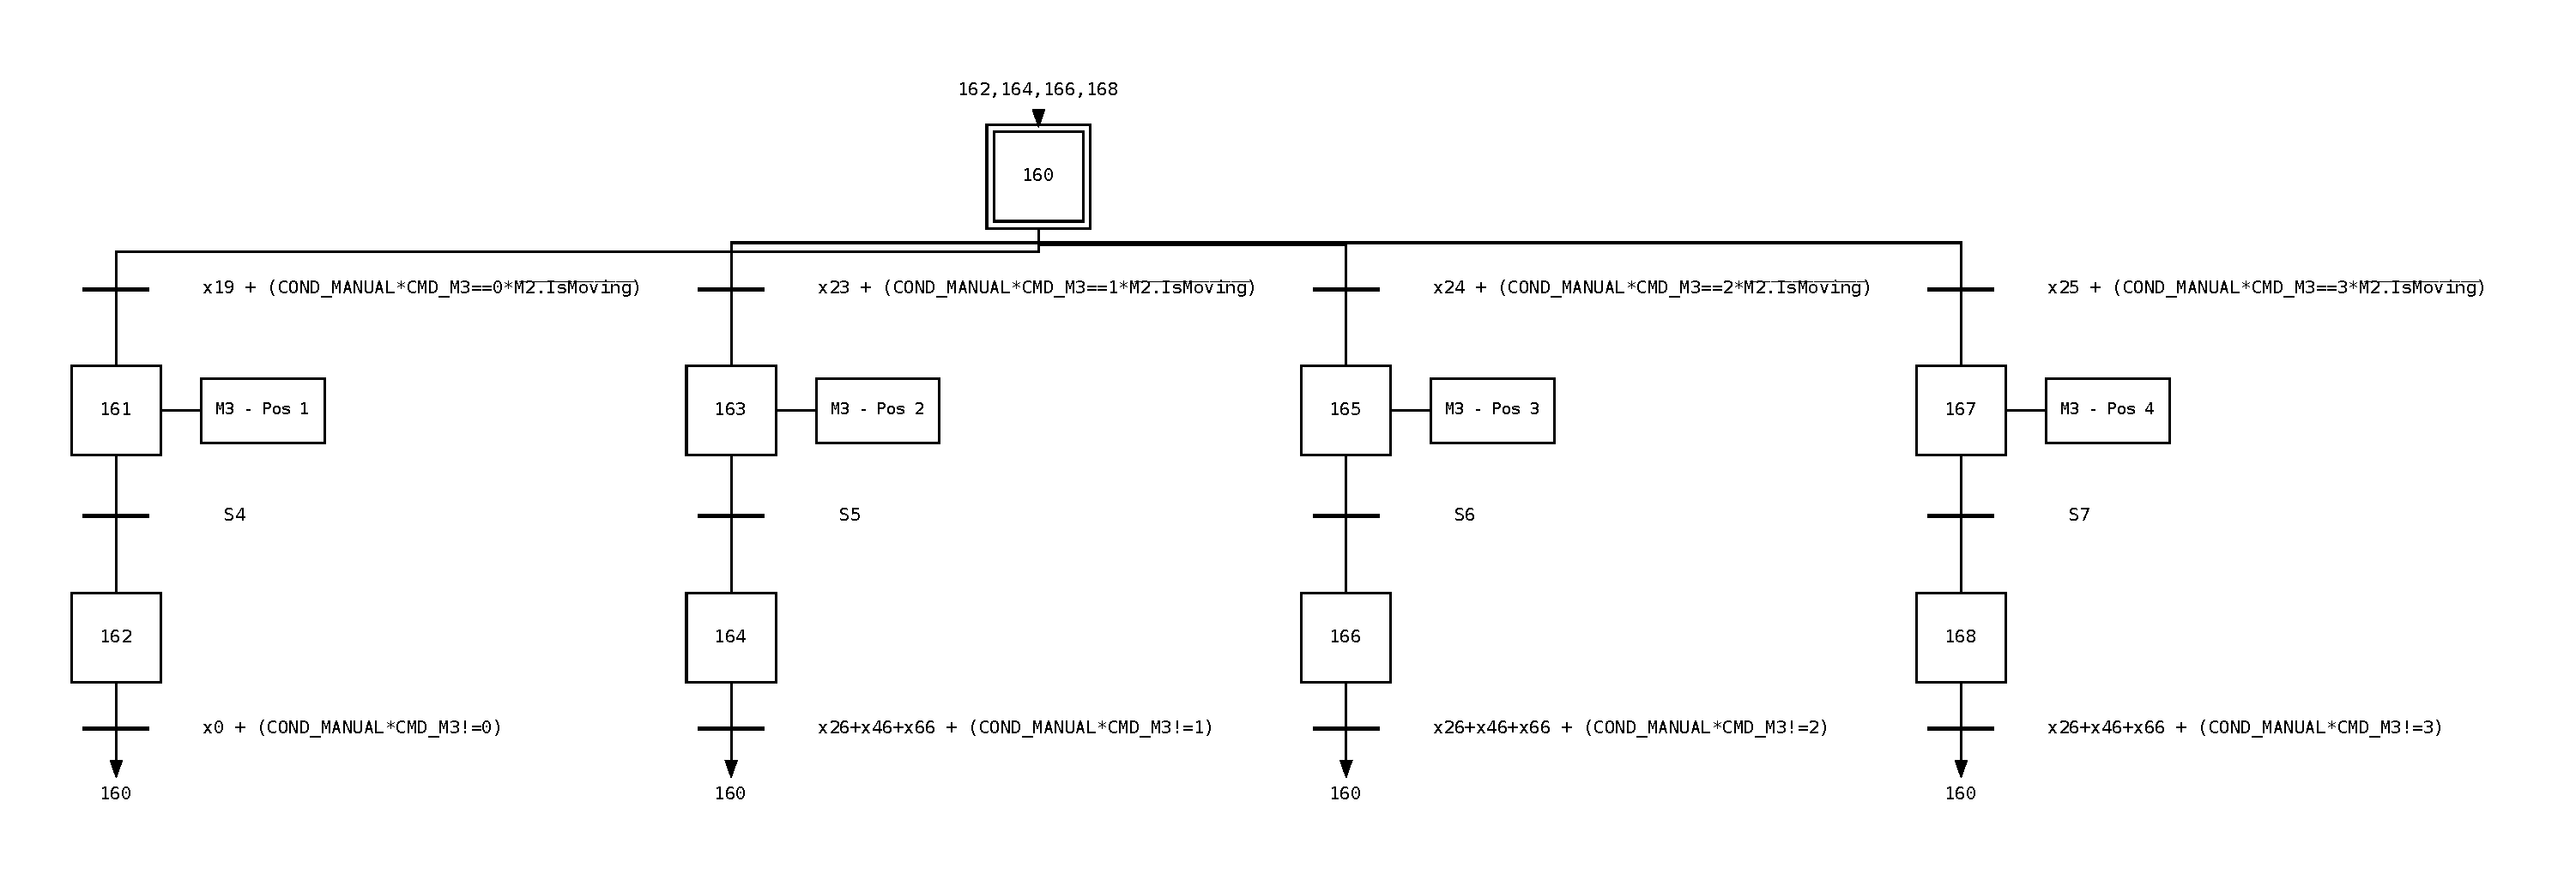
\includegraphics[width=\textwidth]{PDF_GRAFCET/G160.pdf}

\vspace{4pt}
\small (b) Moviment horitzontal
\end{minipage}
\caption{GRAFCETs del transelevador}
\label{fig:grafcet_transelevador}

\end{figure}


\subsection{Grafcet Selector}
\label{section_selector}

Aquest programa (G500, Figura \ref{fig:grafcet_selector}) gestiona el mode de funcionament del sistema, integrant tant la selecció de mode com les condicions de seguretat i transició.

\begin{itemize}
\item \textbf{E500:} Estat de decisió (neutre)
\item \textbf{E501:} Mode automàtic actiu
\item \textbf{E502:} Aturada de mode automàtic
\item \textbf{E503:} Mode manual actiu
\item \textbf{E504:} Aturada de mode manual
\end{itemize}

\textbf{Variables implicades:}
\begin{itemize}
\item Selector: 0 (automàtic), 1 (manual)
\item B\_Start: Botó d'arrencada (Normalment obert)
\item B\_Stop: Botó d'aturada (Normalment tancat)
\item E0: Estat inicial del G0
\item E600: etapa relacionada amb la gesitó d'una aturada d'emergència
\item CI: Condicions inicials del sistema
\item CI\_Actuators: Actuadors en posició segura
\end{itemize}

\textbf{Funcionament:}

\begin{itemize}

\item \textbf{E500 (Decisió):}  
És l'estat inicial on es decideix el mode de funcionament.  
En aquest estat:
\begin{itemize}
\item Si el selector està en posició automàtica (0) i es prem \textbf{B\_Start}, es passa a \textbf{E501}.
\item Si el selector està en posició manual (1) i es prem \textbf{B\_Start}, es passa a \textbf{E503}.
\end{itemize}

\item \textbf{E501 (Mode automàtic):}  
El sistema entra en funcionament automàtic:
\begin{itemize}
\item S'activa la llum de color verd, indicant funcionament automàtic.
\item Es surt d'aquest estat si:
\begin{itemize}
\item Es prem \textbf{B\_Stop} per aturar simplement el sistema, o
\item El selector deixa d'estar en automàtic canviant la direcció i polsant  \textbf{B\_Stop} per validar l'aturada.
\end{itemize}
En aquest cas es passa a \textbf{E502}.
\end{itemize}

\item \textbf{E502 (Aturada del sistema):}  
\begin{itemize}
\item El sistema espera que el G0 torni a l'estat inicial (\textbf{E0 activa}).
\item Un cop assolit, es retorna a \textbf{E500}.
\end{itemize}

\item \textbf{E503 (Mode manual):}  
El sistema entra en mode manual:
\begin{itemize}
\item S'activa la llum de color groga indicant l'entrada en mode manual
\item L'usuari pot controlar directament els actuadors.
\item Es surt d'aquest estat si:
\begin{itemize}
\item El selector deixa d'estar en manual i es prem \textbf{B\_Stop} com a validació, o
\item El GRAFCET s'emergència arriba a una etapa específica de finalització (\textbf{E602 de G600}).
\end{itemize}
En aquests casos es passa a \textbf{E504}.
\end{itemize}

\item \textbf{E504 (Sortida de manual):}  
\begin{itemize}
\item Es verifica que el sistema es troba en condicions segures:
\begin{itemize}
\item Condicions inicials  (\textbf{CI})
\item Actuadors en posició segura (\textbf{CI\_Actuators})
\end{itemize}
\item Un cop complertes, es retorna a \textbf{E500}.
\end{itemize}

\end{itemize}


\begin{figure}[H]
\centering
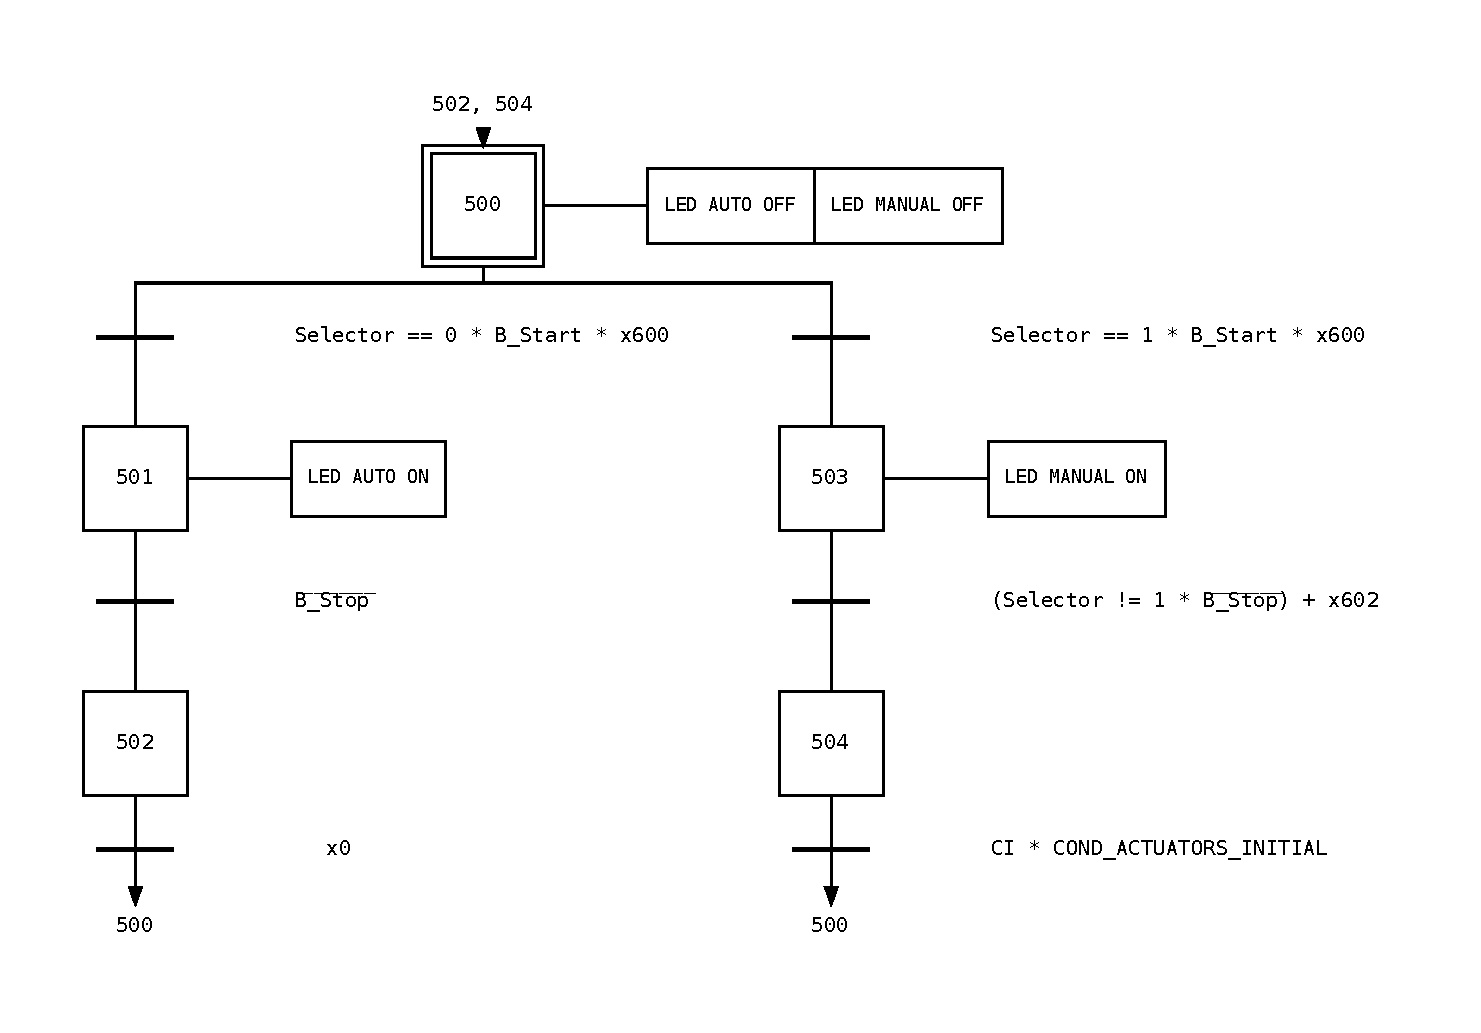
\includegraphics[width=0.7\textwidth]{PDF_GRAFCET/G500.pdf}
\caption{GRAFCET del selector de mode}
\label{fig:grafcet_selector}
\end{figure}
\subsubsection{Grafcet Emergència}

\begin{wrapfigure}[13]{r}{0.36\textwidth}

\vspace{-15pt}

\centering
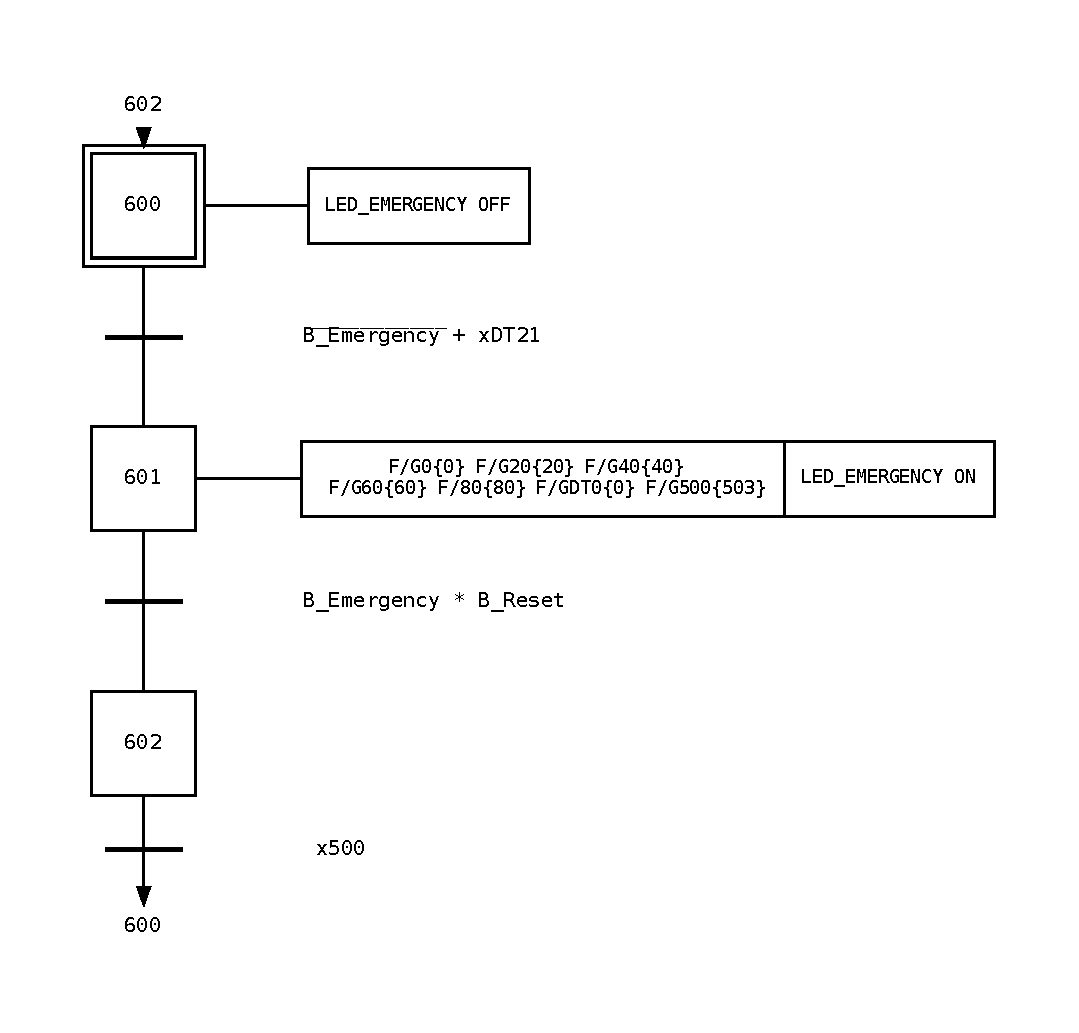
\includegraphics[width=0.5\textwidth]{PDF_GRAFCET/G600.pdf}
\caption{GRAFCET d'emergència}
\label{fig:grafcet_emergencia}

\vspace{-7pt}

\end{wrapfigure}


Aquest G600 (Figura \ref{fig:grafcet_emergencia}) gestiona les situacions d'emergència del sistema i garanteix una aturada segura de tots els processos.

Consta de tres etapes:

\begin{itemize}
\item \textbf{E600:} Estat inicial, no emergència actica
\item \textbf{E601:} El sistema entra en l'estat d'emergència
\item \textbf{E602:} Validació de condicions inicials per sortir del mode d'emergència
\end{itemize}

\paragraph{Activació de l'emergència}

L'activació es pot produir de dues maneres:

\begin{itemize}
\item Mitjançant el botó d'emergència (\textbf{B\_Emergency}), el qual és \textbf{normalment tancat}. Quan es prem, el contacte s'obre i es detecta la situació d'emergència.
\item Mitjançant una condició d'error del sistema, representada per l'activació de l'etapa $xDT21$ del GRAFCET de fallada (dual tween).
\end{itemize}

\paragraph{Comportament en emergència}

Quan el sistema entra en l'estat \textbf{E601}:

\begin{itemize}
\item Es produeix la \textbf{congelació de tots els GRAFCETs}, evitant l'evolució dels programes així com l'aturada de tots els actuadors..
\item Es força el sistema a \textbf{mode manual}, impedint el funcionament automàtic.
\item Es realitza un \textbf{reset de múltiples GRAFCETs}, retornant-los a etapes segures.
\item S'activa una senyalització visual (LED d'emergència).
\end{itemize}

Aquest comportament assegura que la planta es mantingui en un estat segur independentment del punt del procés en què es trobava.

\paragraph{Sortida de l'emergència}

Per sortir de l'estat d'emergència cal complir dues condicions:

\begin{itemize}
\item El botó d'emergència ha de tornar a la seva posició normal (contacte tancat).
\item S'ha de prémer el botó de reset (\textbf{B\_Reset}).
\end{itemize}

Aleshores el sistema passa a \textbf{E602}, on es verifica si el sistema compleix les condicions inicials.Un cop complert, es retorna a \textbf{E600}.

Això evita reinicis perillosos i garanteix que el sistema es reprengui únicament des d'una situació controlada.




\subsubsection{Detecció d'avaries}

\begin{wrapfigure}[24]{r}{0.45\textwidth}

\vspace{-10pt}

\centering
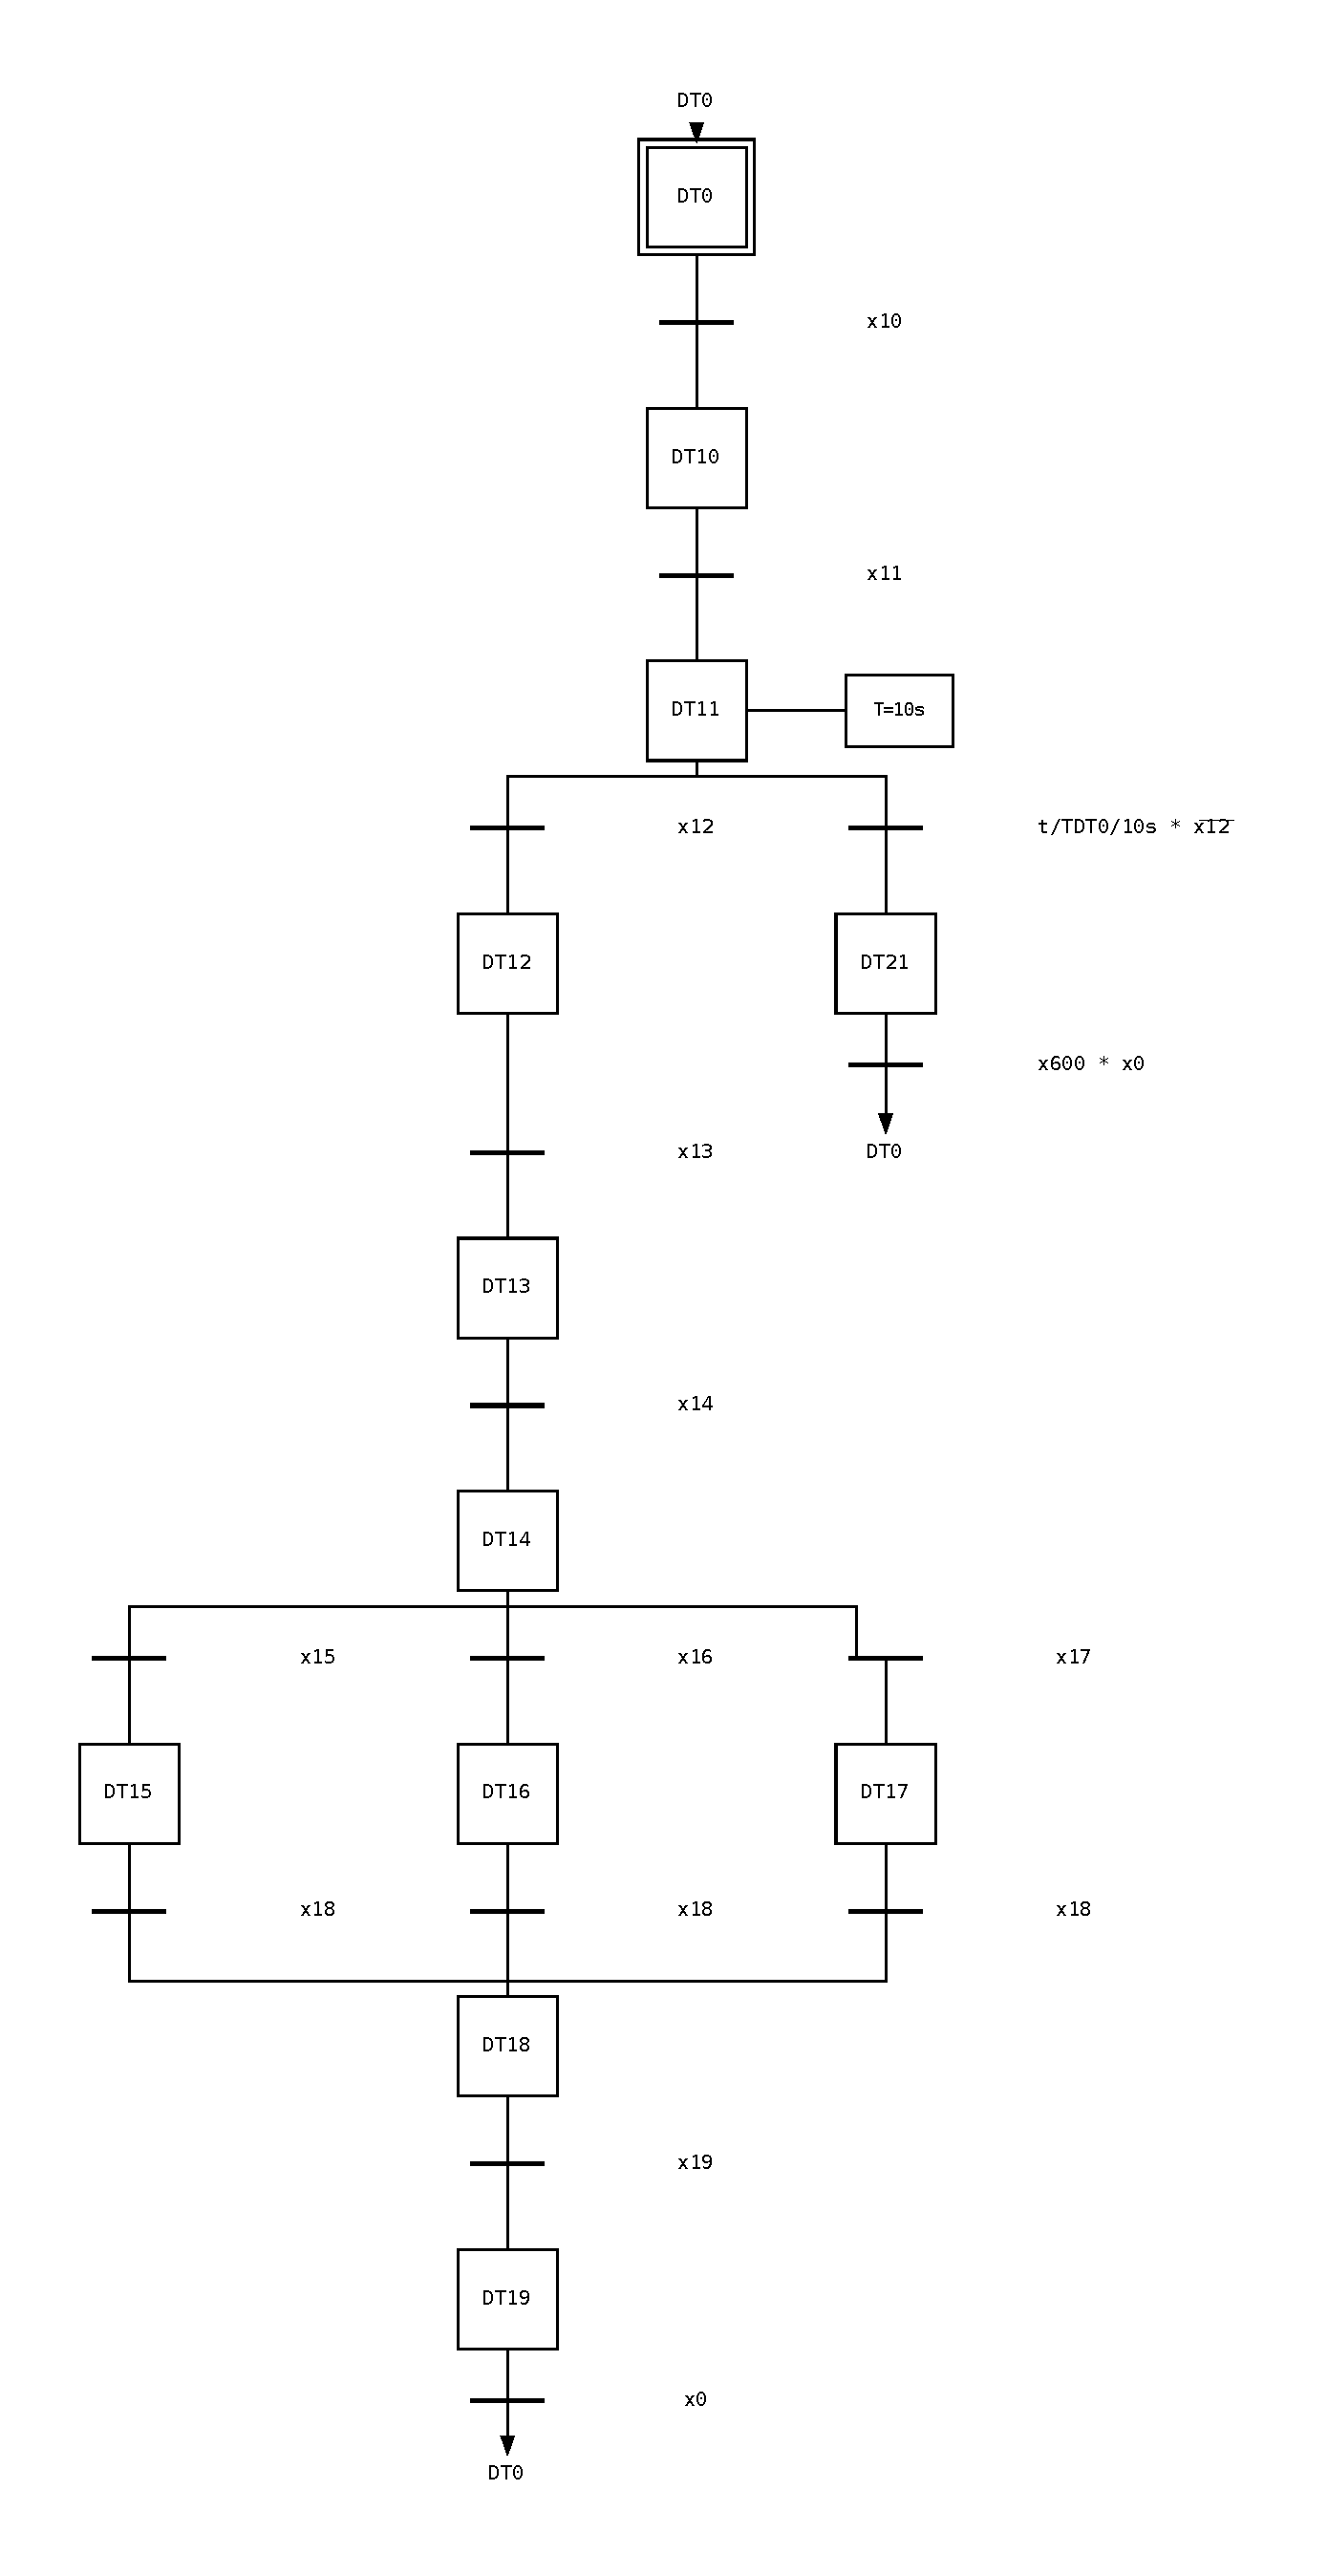
\includegraphics[width=0.5\textwidth]{PDF_GRAFCET/GDT0.pdf}
\caption{Grafcet d'avaria (Dual TWEEN)}
\label{fig:grafcet_avaria}

\vspace{-5pt}

\end{wrapfigure}

El GRAFCET d'avaria es basa en un sistema de supervisi temporal implementat mitjançant un \textbf{Dual TWEEN} (GDT0, Figura \ref{fig:grafcet_avaria}). Aquest programa permet detectar situacions en què una transició del procés no es completa dins d'un temps esperat, indicant una possible fallada del sistema.

\paragraph{Funcionament general}

El programa de detecció d'avaria segueix el mateix flux que el GRAFCET general en la seva fase inicial, especialment en la part de detecció de la peça. Això permet monitoritzar en paral·lel el correcte funcionament del procés.

\paragraph{Condició d'activació de l'avaria}

L'avaria es produeix quan el sistema no és capaç de determinar el tipus de peça dins d'un temps límit establert.

Concretament, això passa quan la peça ha estat detectada en entrada (activació de S1), però el sensor \textbf{S2} no identifica el tipus de peça (A, B o C) en un temps superior a \textbf{10 segons}.

Si aquesta condició es compleix, el sistema considera que existeix una fallada en la detecció i activa el GRAFCET d'avaria \footnote{Aquesta fallada està forçada dintre de Unity per part meva per tal d'observar com actua el sistema en aquests tipus de situacions.}.  Quan el temps màxim és superat en l'etapa \textbf{EDT11}, es produeix la transició cap a l'estat \textbf{EDT21}.



Aquest estat té com a funció principal activar directament el \textbf{GRAFCET d'emergència}, provocant tot el que s'ha explicat en l'apartat anterior del grafcet d'emergència (congelació de processos, mode manual, reset de grafcets, etc).

\paragraph{Sortida de l'estat d'avaria}

La sortida d'aquest estat no es realitza de forma automàtica, sinó que queda condicionada al procés de recuperació del GRAFCET d'emergència, amb la diferència que en aquest cas, l'operari ha de revisar la causa de l'error abans de presionar el botó de RESET (el botó d'emergència en teoría ja esta en la posició correctar al saltar aquesta avaria automàticament). .






\section{Implementació del control en Unity}
Per a la simulació del sistema industrial s'ha desenvolupat un script principal anomenat \texttt{PlantController}, el qual actua com a nucli de control de tota la planta dins de Unity.

Aquest script conté totes les variables públiques associades als elements del sistema, incloent sensors, actuadors, comptadors i sistemes auxiliars, permetent així una integració completa del model digital amb la lògica de control basada en GRAFCET.

\subsection{Estructura general del controlador}

El controlador es basa en una arquitectura centralitzada on tots els GRAFCETs s'executen de manera simultània dins del mètode \texttt{Update()}, el qual s'executa a cada frame del motor de Unity.

\begin{itemize}
\item Cada GRAFCET està implementat com una funció independent
\item Tots els GRAFCETs són cridats seqüencialment a cada iteració del cicle
\item Es requereix un control rigorós de les condicions per evitar conflictes entre processos simultanis
\end{itemize}

\begin{lstlisting}[language=C]
void Update() {
  GRAFCET_EMERGENCIA();
  GRAFCET_MODO();

  Classification();
  Classification_DUALTWEEN();
  ShelfA();
  ShelfB();
  ShelfC();
  Evacuation();

  GRAFCET_M1();
  GRAFCET_M4();
  GRAFCET_M2();
  GRAFCET_M3();
  GRAFCET_M9_A();
  GRAFCET_M9_B();
  GRAFCET_M9_C();
  GRAFCET_M7();
  GRAFCET_M5();
  GRAFCET_M6();
  GRAFCET_M8();
}
\end{lstlisting}

Es pot observar com tots els GRAFCETs s'executen de forma concurrent, sent el GRAFCET d'emergència el primer en ser avaluat.

\subsection{Gestió d'estats mitjançant variables ETAPA}

Cada GRAFCET es representa mitjançant una variable de tipus enter (\texttt{int}), la qual indica l'etapa activa.

\begin{lstlisting}[language=C]
public int ETAPA_0 = 0; 
public int ETAPA_20 = 20;
public int ETAPA_40 = 40;
public int ETAPA_60 = 60;
public int ETAPA_80 = 80;

public int ETAPA_100 = 100; // M1
public int ETAPA_140 = 140; // M2
public int ETAPA_160 = 160; // M3

public int ETAPA_500 = 500; // SELECTOR
public int ETAPA_600 = 600; // EMERGENCIA
\end{lstlisting}

Cada valor representa una etapa concreta del GRAFCET, i els canvis d'estat es realitzen mitjançant estructures \texttt{switch-case}.

\begin{lstlisting}[language=C]
  void GRAFCET_M1() {
    switch (ETAPA_100) {
    case 100: 
      M1.SetState(false);
      if (ETAPA_0 == 10 || ETAPA_0 == 12 || (COND_MANUAL && CMD_M1 == 1)) ETAPA_100 = 101;
      break;
    case 101: 
      M1.SetState(true);
      if (ETAPA_0 == 11 || ETAPA_0 == 13 || (COND_MANUAL && CMD_M1 == 0)) ETAPA_100 = 100;
      break;
    }
  }
}
\end{lstlisting}

\subsubsection{Sensors i actuadors}

Els sensors i actuadors es defineixen com a variables públiques dins del controlador segons les classes que s'han creat en la resta de scripts:

\begin{lstlisting}[language=C]
public PrescenceSensor S1, S3, S12;
public OpticalSensor S2;

public MotorBelt M1, M8;
public ASRSVertical M2;
public ASRSHorizontal M3;
\end{lstlisting}

Això permet connectar directament els objectes de Unity amb la lògica de control.


\subsection{Gestió de botons}

Els botons es defineixen amb comportament industrial:

\begin{lstlisting}[language=C]
public bool B_Start = false;     // Normalment obert
public bool B_Stop = true;       // Normalment tancat
public bool B_Emergency = true;  // Normalment tancat
public bool B_Pause = false;
public bool B_Reset = false; 
\end{lstlisting}

Aquest model permet simular el comportament real d'una instal·lació industrial.

\subsection{Gestió temporal}

Els temporitzadors permeten controlar retards i detectar errors:

\begin{lstlisting}[language=C]
Timer T0, T1, TDT0;
void Start() {
  T0 = new Timer {preset = 0.15f};
  T1 = new Timer {preset = 1f};
  TDT0 = new Timer {preset = 10f};
}
\end{lstlisting}

Especialment, el temporitzador \texttt{TDT0} s'utilitza per detectar errors en la classificació.

\subsection{Detecció d'errors (Dual TWEEN)}

\begin{lstlisting}[language=C]
case 11:
  TDT0.Update(true);

  if (ETAPA_0 == 12) {
    ETAPA_DT0 = 12;
    TDT0.Update(false);
  }
  else if (TDT0.done) {
    ETAPA_DT0 = 21; // ERROR
  }
  break;
\end{lstlisting}

Si la peça no es detecta en menys de 10 segons, es genera un estat d'error.
\subsection{Control global del sistema: Selector de mode i Emergència}

En la versió actual del sistema s'ha eliminat el GRAFCET específic de \textbf{marxa}, integrant la seva funcionalitat dins del \textbf{selector de mode}. D'aquesta manera, el control global es basa en dos GRAFCETs principals: el \textbf{selector de mode} (G500) i el \textbf{GRAFCET d'emergència} (G600), executats en cada iteració del mètode \texttt{Update()}.

\subsubsection{GRAFCET de selector de mode (ETAPA\_500)}

Aquest GRAFCET centralitza tant la selecció del mode de funcionament com l'activació general del sistema. Els elements de control associats són \texttt{B\_Start}, \texttt{B\_Stop} (normalment tancat) i el\texttt{Selector}de mode (\texttt{0} automàtic, \texttt{1} manual, \texttt{-1} neutre)

Per passar d'un estat a un altre és la mateixa explicació que s'ha explicat en la secció \ref{section_selector}

\subsubsection{GRAFCET d'emergència (G600)}

El GRAFCET d'emergència té la màxima prioritat dins del sistema i pot interrompre qualsevol altre procés en execució.

\paragraph{Activació de l'emergència}

L'emergència es pot activar en dues situacions:
\begin{itemize}
\item Quan es prem el botó \texttt{B\_Emergency} (botó normalment tancat)
\item Quan es detecta una avaria en el sistema de classificació (\texttt{ETAPA\_DT0 = 21})
\end{itemize}

\paragraph{Comportament en emergència (ETAPA 601)}

Quan s'activa l'emergència:
\begin{itemize}
\item Es desactiva el funcionament normal del sistema (\texttt{LS.isOk = false})
\item S'activa la senyalització d'emergència (\texttt{LS.emergency = true})
\item Es reinicien tots els GRAFCETs del procés automàtic mitjançant \texttt{ResetGrafcetsProcess()}
\item Es força el sistema a mode manual (\texttt{ETAPA\_500 = 503})
\end{itemize}

Aquest comportament assegura una aturada immediata i segura davant qualsevol situació anòmala.

\paragraph{Sortida de l'emergència}

La recuperació del sistema requereix una acció conscient per part de l'operador. Per sortir de l'estat d'emergència és necessari:

\begin{itemize}
\item Que el botó d'emergència torni a la seva posició normal
\item Prémer el botó de \texttt{reset} (\texttt{B\_Reset})
\end{itemize}

Això provoca la transició a l'estat \textbf{ETAPA 602} (reset d'emergència).

Finalment, el sistema només retorna a l'estat inicial (ETAPA 600) quan:
\begin{itemize}
\item El selector de mode també ha tornat a una situació vàlida (ETAPA\_500 = 500)
\end{itemize}

\subsection{Control manual dels actuadors}

\begin{lstlisting}[language=C]
public int CMD_M1 = 0;
public int CMD_M2 = -1;
public int CMD_M3 = -1;
\end{lstlisting}

Aquestes variables permeten controlar manualment els actuadors en mode manual. Els valors s'actualitzaren a través dels tòpics MQTT, provenent del RapidScada. També és necessari que la condició de COND\_MANUAL estigui activa a part de modificar aquestes variables de CMD. 

Pel que fa als transelevadors, tal i com hem explicat previàment. , quan el transelevador arriba a la posició inicial, la comanda s'ha de forçar a un valor neutre (\texttt{-1}), evitant que el sistema torni a executar automàticament el mateix moviment.

D'altra banda, en els estats de confirmació, la condició de sortida inclou explícitament que la comanda sigui diferent de la que ha originat el moviment, assegurant així que només una nova ordre provoca un canvi d'estat.

A més, es tenen en compte condicions addicionals com:
\begin{itemize}
\item La sincronització amb altres GRAFCETs del procés automàtic
\item La verificació que altres eixos no estiguin en moviment simultàniament
\end{itemize}

\subsection{Sistema de reset}

\begin{lstlisting}[language=C]
void ResetGrafcetsProcess() {
  ETAPA_0 = 0;
  ETAPA_20 = 20;
  ETAPA_40 = 40;
  ETAPA_60 = 60;
  ETAPA_80 = 80;
}
\end{lstlisting}

Aquest mecanisme garanteix que el sistema torna a un estat segur després d'una emergència.

\subsection{Gestió avançada de senyals i control intern}

Per tal de garantir un comportament robust i fiable del sistema, s'han implementat diversos mecanismes interns de control que complementen la lògica GRAFCET. Aquests inclouen la detecció de flancs, la gestió de comptadors, els resets controlats i la integració amb el sistema d'avaries.

\subsubsection{Detecció de flanc de pujada amb diccionari (Rising Edge)}

En aquest sistema, la detecció de flanc de pujada (rising edge) no es realitza mitjançant variables individuals, sinó a través d'un \textbf{diccionari d'estats previs}, que permet gestionar múltiples senyals de forma escalable i organitzada.

\begin{lstlisting}[language=C]
Dictionary<string,bool> prevStates=new Dictionary<string, bool>();

bool RisingEdge(string key, bool current){
  bool prev = false;
  if (prevStates.ContainsKey(key))prev = prevStates[key];
  prevStates[key] = current;
  return current && !prev;
}
\end{lstlisting}

\paragraph{Funcionament}

El funcionament es basa en associar cada senyal a una \textbf{clau única} (\texttt{key}) dins del diccionari:

\begin{itemize}
\item \textbf{key}: identifica la senyal (per exemple, una etapa concreta d'un GRAFCET)
\item \textbf{current}: valor actual de la condició
\item \textbf{prev}: valor anterior emmagatzemat al diccionari
\end{itemize}

El procés és el següent:

\begin{enumerate}
\item Es consulta el valor anterior de la senyal dins del diccionari
\item Si no existeix, s'assumeix com a \texttt{false}
\item S'actualitza el diccionari amb el valor actual
\item Es retorna \texttt{true} només si la senyal ha passat de 0 a 1
\end{enumerate}

Això permet detectar de forma precisa el moment exacte en què una condició s'activa.

\paragraph{Ús dins dels GRAFCETs}

Cada flanc de pujada es defineix amb una clau única associada a una etapa concreta. Per exemple:

\begin{lstlisting}[language=C]
if (RisingEdge("ETAPA_0_10", ETAPA_0 == 10))
  Spawner.SpawnPiece();
\end{lstlisting}

En aquest cas, l'acció només s'executa una vegada en entrar a l'etapa 10, evitant execucions repetides a cada frame.

Com podreu observar, aquestta funció implementada per mi de Rising\_Edge s'ha aplicat tant per introduir una peça en l'etapa que toca com modificar el valors dels 6 comptadors que hi ha dintre del sistema en les etapes corresponent. Com únicament és necessari fer-ho quan s'activa l'etapa, aquesta funció és perfecta per aquestes situacions.

\paragraph{Reinicialització obligatòria}

És fonamental reinicialitzar l'estat del diccionari per cada clau quan es torna a l'etapa inicial del GRAFCET. En cas contrari, el sistema podria no detectar correctament futurs flancs.

\begin{lstlisting}[language=C]
case 0:
  prevStates["ETAPA_0_10"] = false;
  if (COND_AUTO && CI) ETAPA_0 = 10;
  break;
\end{lstlisting}

Aquesta reinicialització garanteix que, quan el GRAFCET torni a començar, el flanc de pujada es detectarà correctament de nou.



\end{document}

